\documentclass{article}
\usepackage[utf8]{inputenc}
\usepackage[margin = 0.8in]{geometry}
\usepackage{graphicx}
\usepackage{amsmath, amssymb}
\usepackage{subcaption}
\usepackage{multirow}
\usepackage{mathtools}
\usepackage{float}


\title{RBE502 - Homework Set 10}
\author{Keith Chester}
\date{Due date: November 17 2021}

\begin{document}
\maketitle

\section*{Introduction}

In this homework set we aim to create a control system for a 2 link sanding robot arm. The control system will utilize feedback linearization and impedance control in order to create the specified sanding motion per the problem.


\begin{figure}[H]
    \centering
    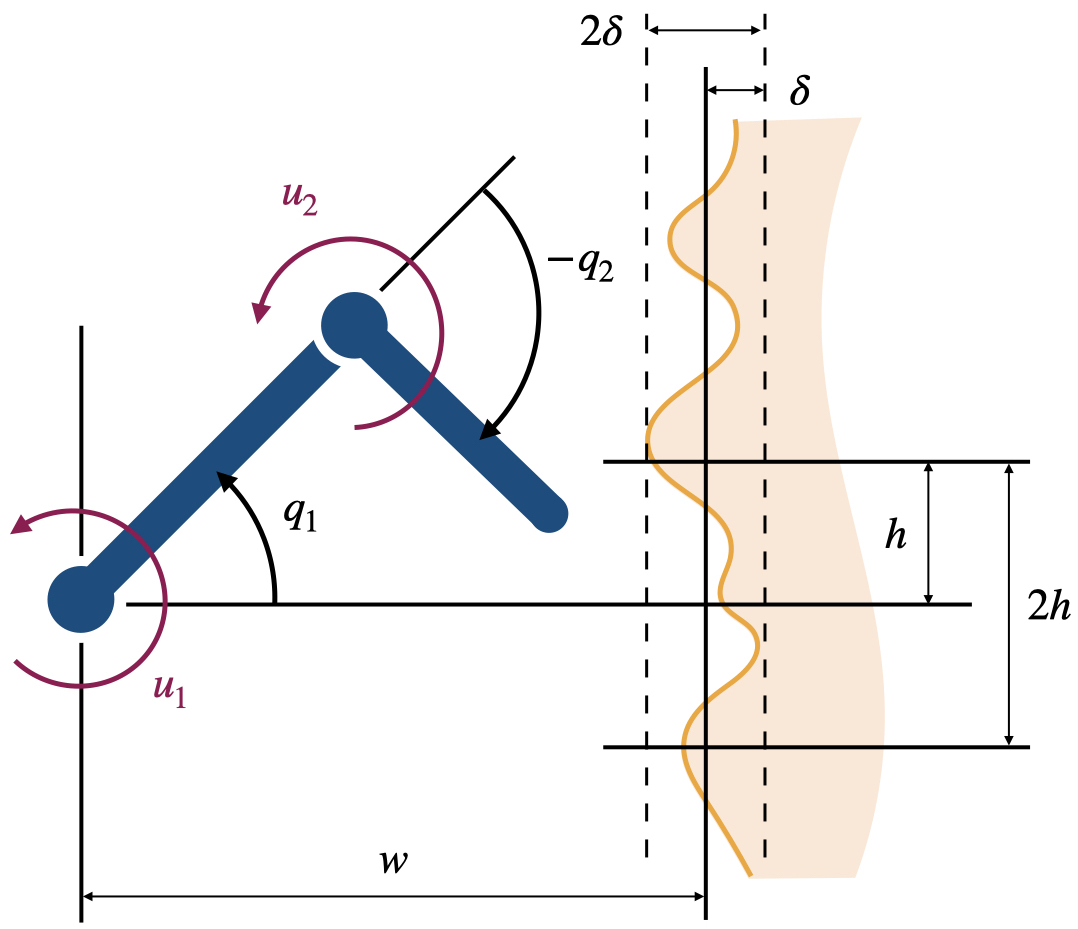
\includegraphics[width = 0.5\textwidth]{figures/arm_impedance_homework.jpeg}
    \caption{2 link robot arm for sanding}
    \label{fig:arm}
\end{figure}

We are assuming that the center of mass for each link is located at the end of the link for simplicity. This results in the mass moment of inertia for the links being zero. This allows us to model the robot arm as a double pendulum system.

\begin{figure}[H]
    \centering
    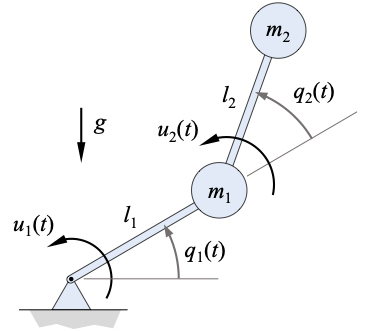
\includegraphics[width = 0.5\textwidth]{figures/doublependulum.jpg}
    \caption{Double pendulum system diagram}
    \label{fig:system-diagram}
\end{figure}

With this system, we can model our system with a differential equation of motion. With $\boldsymbol{q} = \begin{bmatrix} q_1 & q_2 \end{bmatrix}^T$, $\boldsymbol{u} = \begin{bmatrix} u_1 & u_2 \end{bmatrix}^T$, we can define the system as:

\begin{equation}
    M(\boldsymbol{q})\boldsymbol{\ddot{q}} + \phi(\boldsymbol{q}, \boldsymbol{\dot{q}}) = \boldsymbol{u}
\end{equation}

\begin{equation}
    M(\boldsymbol{q}) = \begin{bmatrix}
        (m_1+m_2)l_1^2+m_2 l_2^2 + 2 l_1 l_2 m_2 \cos(q_2) & m_2l_2(l_1 \cos(q_2) + l_2) \\
        m_2 l_2 (l_1 \cos(q_2)+l_2) & m_2 l_2^2
    \end{bmatrix}
\end{equation}

\begin{equation}
    \phi(\boldsymbol{q}, \boldsymbol{\dot{q}}) = \begin{bmatrix}
        (m_1+m_2)gl_1 \cos(q_1) + m_2 l_2 (g \cos(q_1+q_2) - l_1 \dot{q}_2(2\dot{q}_1+\dot{q}_2)\sin(q_2)) \\
        m_2 l_2  (l_1 \dot{q}_1^2 \sin(q_2) + g \cos(q_1 + q_2))
    \end{bmatrix}
\end{equation}

We will be assuming that the horizontal distance of the wall from the base of the robot is measured in $w = \frac{l_1 + l_2}{2}$. We aim to sand a vertical segment of the wall at a distance $h = \frac{l_1+l_2}{3}$. The surface of the wall has irregularities $\sigma = \frac{l_1+l_2}{10}$. Our sanding force is expected to be $5 N \leq r_x \leq 7 N$.

For simulation purposes, assume that we have the values of $m_1 = 2kg$, $m_2 = 1kg$, $l_1 = 1$, $l_2=1$, and $g = 9.81\frac{m}{s^2}$.

\section*{Deriving Equations}

To tackle this problem we will be looking to derive the necessary equations for our system to build our controller. First we will solve the forward kinematics of our arm - for a given state $\boldsymbol{q}$ what is the position of our end effector, $\boldsymbol{z}$. Thus:

\begin{equation}
    \boldsymbol{z} = \begin{bmatrix}
        l_2 \cos(q_1+q_2) + l_1 \cos(q_1) \\
        l_2 * sin(q_1 + q_2) + l_1 \sin(q_1)
    \end{bmatrix}
\end{equation}

With this state variable $\boldsymbol{z}$ we can solve for its Jacobian $\boldsymbol{J}$ via:

\begin{equation}
    \boldsymbol{J} = \begin{bmatrix}
        \frac{\partial z_1}{\partial q_1} & \frac{\partial z_1}{\partial q_2} \\[1em]
        \frac{\partial z_2}{\partial q_1} & \frac{\partial z_1}{\partial q_2}
    \end{bmatrix}
\end{equation}

\begin{equation}
    \boldsymbol{J} = \begin{bmatrix}
        -l_2 \sin(q_1 + q_2) - l_1 \sin(q_1) & -l_2 \sin(q_1 + q_2) \\
        l_2 \cos(q_1 + q_2) + l_1 \cos(q_1) & l_2 \cos(q_1 + q_2)
    \end{bmatrix}
\end{equation}

We know that $\boldsymbol{\dot{z}} = J(q) \dot{q}$, but we need $\boldsymbol{\ddot{z}}$. This would require us to find $\dot{J}$, which is the time derivative of the Jacobian. We find this via:

\begin{equation}
    \boldsymbol{\dot{J}} = \begin{bmatrix}
        \frac{d}{dt} \left( -l_2 \sin(q_1 + q_2) - l_1 \sin(q_1))\right) & \frac{d}{dt} \left( -l_2 \sin(q_1 + q_2)\right) \\
        \frac{d}{dt} \left( l_2 \cos(q_1 + x_2) + l_1 \cos(q_1)\right) & \frac{d}{dt} \left( l_2 \cos(q_1 + q_2) \right)
    \end{bmatrix}
\end{equation}

\begin{equation}
    \boldsymbol{\dot{J}} = \begin{bmatrix}
        -\dot{q}_1 (l_2 \cos(q_1 + q_2) + l_1 \cos(q_1) - \dot{q}_2 l_2 \cos(q_1 + q_2)) &  -l_2 \cos(q_1 +q_2)(\dot{q}_1 + \dot{q}_2) \\
        - \dot{q}_1 (l_2 \sin(q_1 + q_2) + l_1 \sin(q_1)) - \dot{q}_2 l_2 \sin(q_1 + q_2) & -l_2 \sin(q_1 +q_2) (\dot{q}_1 + \dot{q}_2)
    \end{bmatrix}
\end{equation}
     
Solving for our $\boldsymbol{\ddot{z}}$ from the equation $\boldsymbol{\dot{z}} = J(q) \dot{q}$, we get a resulting equation $\boldsymbol{\ddot{z}} = J(q) \ddot{q} + \dot{J}(q) \dot{q}$. To isolate and solver for $\ddot{q}$, we then get:

\begin{equation}
    \ddot{q} = J^{-1}(q) \left( \ddot{z} - \dot{J}(q)\dot{q}  \right)
\end{equation}

The equation we utilize for a system represented as a mass spring damper system is $M_e \ddot{z} + B \dot{z} + K(z-z_0) = r$. Isolating the $\ddot{z}$ we have $\ddot{z} = M_e^{-1}\left( r - B \dot{z} - K(z-z_0) \right)$. Utilizing this value in our $\ddot{q}$ derivation, we have:

\begin{equation}
    \ddot{q} = J^{-1}(q) \left( M_e^{-1}\left( r - B \dot{z} - K(z-z_0) \right) - \dot{J}(q)\dot{q}  \right) 
\end{equation}

\end{document}